\section{Fase 1: Mapa de preguntas sobre el cáncer de mama (BCQM)} 
En esta fase se propone el uso de un mapa de preguntas sobre el cáncer de mama (BCQM). El proposito del \textit{BCQM} es que el \textit{Data Analysis Team} defina las preguntas que serán resueltas al finalizar cada \textit{Release} y que permitirán tomar decisiones medicas con respecto al diagnostico de esta enfermedad. En la figura \ref{BCQM} se observa la estructura del BCQM.

\begin{figure}
	\centering
	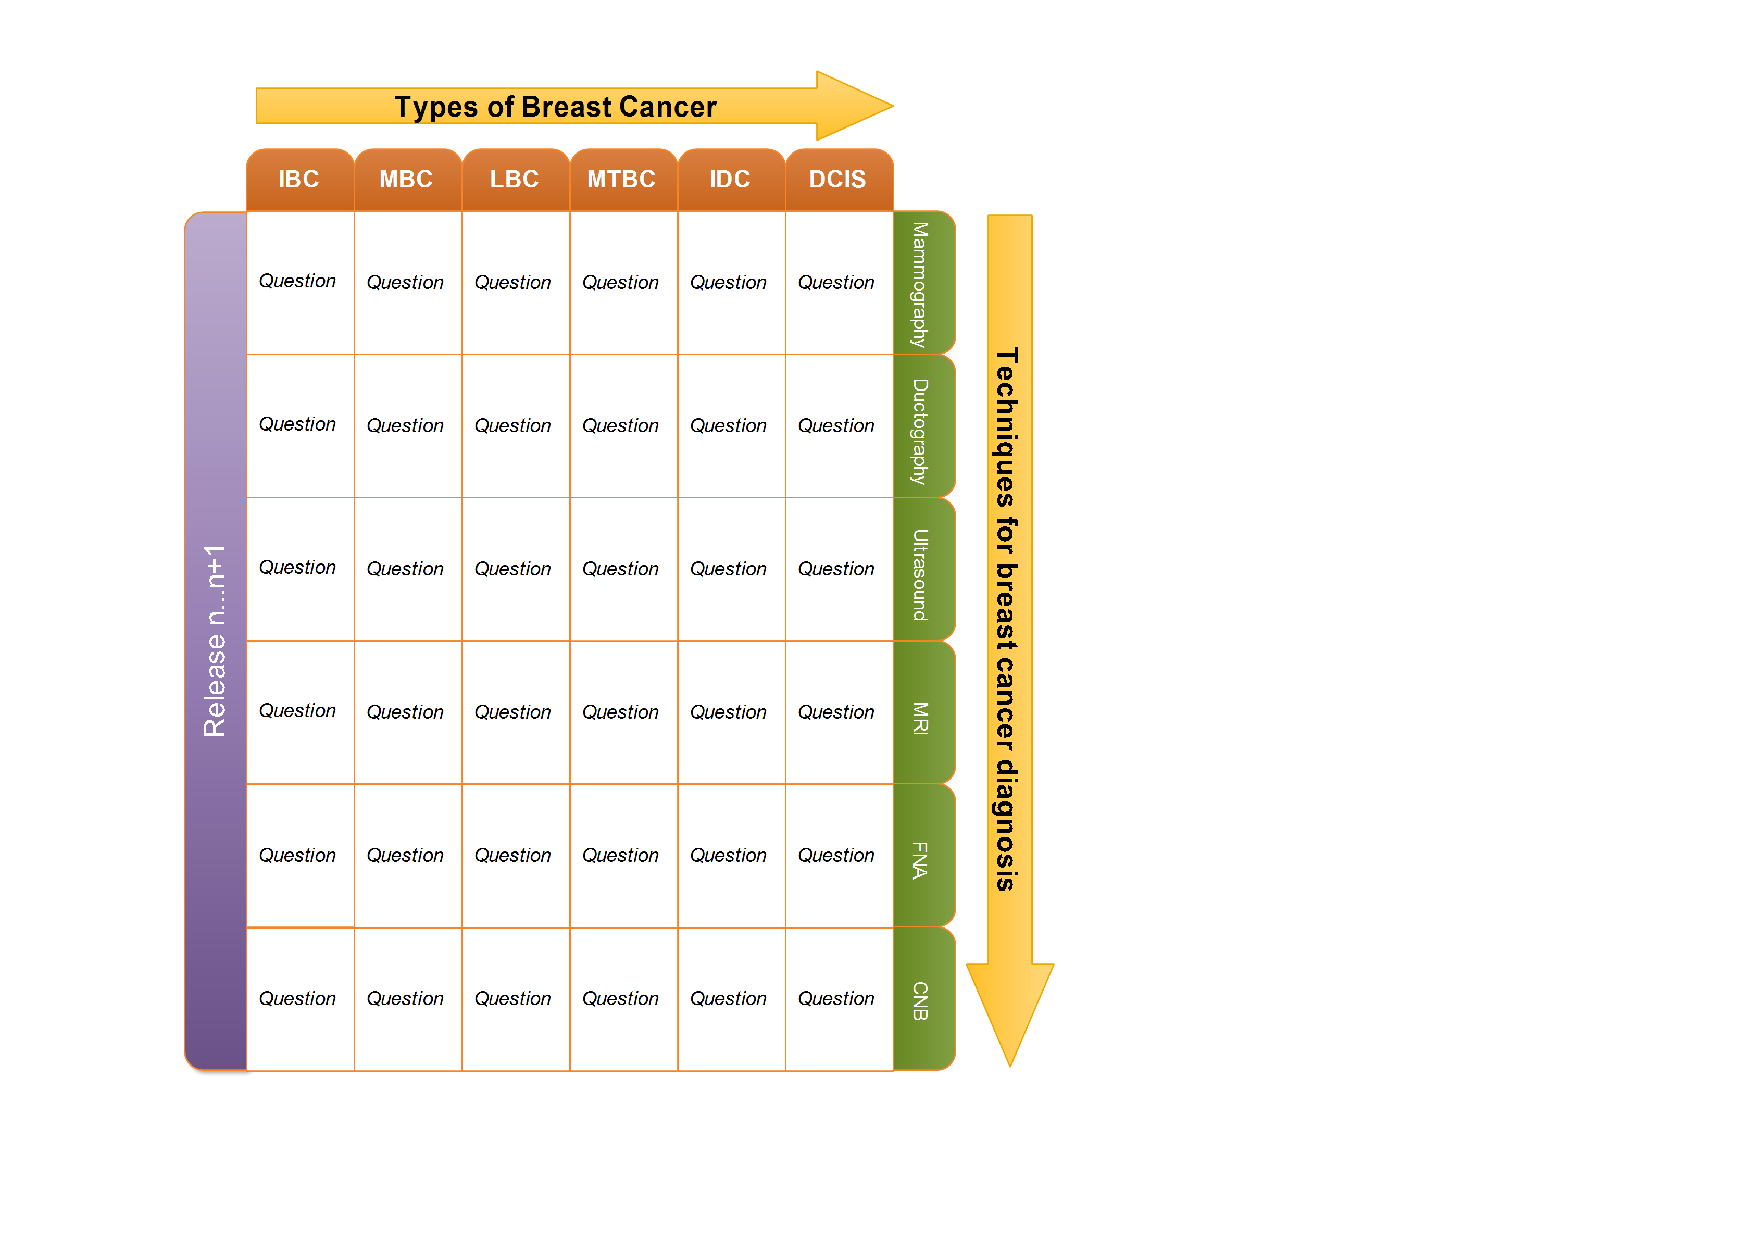
\includegraphics[width=0.6
	\linewidth]{IMAGENES/BCQM}
	\caption{Mapa de preguntas basados en los tipos de cáncer de mama \textit{inflamatorio (IBC)}, \textit{mucinoso (MBC)}, \textit{Lobulillar (LBC)}, \textit{Tumores mixtos (MTBC)}, \textit{Carcinoma ductal invasivo (IDC)} y \textit{Carcinoma ductal in situ (DCIS)}}
	\label{BCQM}
\end{figure}

El BCQM permite plantear preguntas relacionadas a los tipos de cáncer de mama y a las técnicas para el diagnostico de la misma. De modo que al finalizar el tiempo de cada \textit{Release}, el cual puede variar entre 1 y 4 semanas, las preguntas serán respondidas según el análisis de datos generado, y el medico podrá tomar una decisión de valor. Cabe resaltar, que es posible tener una o mas preguntas relacionadas a una técnica y a un tipo de cáncer de mama por cada \textit{Release}, razón por la cual es posible encontrar correlaciones entre las variables características de cada tipo de cáncer encontrando así patrones ocultos en los diferentes conjuntos de datos. Adicionalmente, el BCQM permite identificar a que técnica para el diagnostico de cáncer mama esta relacionada la pregunta a resolver, lo cual de antemano hace posible conocer el tipo información (imágenes o datos) y el algoritmo  ML o DL requerido para dar solución al problema. Así mismo, el BCQM permite definir desde la fase inicial el tipo de modelo predictivo o descriptivo según el enfoque analítico generado por la pregunta planteada. Sintetizando, el uso de BCQM facilita la comprensión del problema medico y permite identificar previamente la técnica, el tipo de información y enfoque que debe ser utilizado para el análisis de datos.  